\chapter{HTML简介}

\section{前后端}

\subsection{前端工程师(Front-End Engineer)}

前端工程师互联网时代软件产品研发中不可缺少的一种专业研发角色。前端是一个相对比较新的行业,大约从2005年开始,正式的前端工程师角色被行业所认可。到了2010年,互联网开始全面进入移动时代,前端工程师的地位也越来越重要。 \\

现在一些后端开发工作也可以由前端工程师来完成。最初所有的开发工作都是由后端工程师完成的,但是随着业务越来越繁杂、工作量过大,后端工程师们不堪重负,于是将可视化和部分交互功能的开发剥离出来,形成了前端开发。 \\

前端工程师主要负责的工作就是使用HTML、CSS、JavaScript等专业技能和工具将产品UI设计稿实现成网站产品。涵盖用户PC端和移动端网页,处理视觉和交互问题。 \\

广义上讲,所有用户终端产品,只要是与视觉和交互有关的部分都是前端工程师的专业领域。产品从前期开发到后期的维护、更新、升级都需要前端工程师来完成。

\subsection{后端工程师(Back-End Engineer)}

后端工程师主要负责服务器的数据逻辑和业务逻辑等,主要研究怎么把数据更好地传输给前端工程师。 \\

如果一个人除了完成前端开发和后端开发工作以外,从产品设计到项目开发,再到后期运维都是同一个人,甚至可能还要负责UI、配动画、写文档等,那么就被称为全栈工程师(Full Stack Engineer)。

\subsection{前端应用领域}

前端技术可以被应用在一系列领域中:

\begin{itemize}
    \item 网页网站
    \item APP、微信小程序
    \item 移动端小游戏
    \item 炫酷的特效
    \item 大数据可视化
    \item VR虚拟现实
\end{itemize}

前端工程师需要具备大量必要的技能,其中前端三大基础语言为HTML、CSS、JavaScript,除此之外还需要学习jQuery、网络、es6、webpack4.0、小程序、VUE、React、Node.js、Mongo DB数据库等内容。 \\

\newpage

\section{结构层/表现层/行为层}

\subsection{结构层/表现层/行为层}

\begin{itemize}
    \item 结构层HTML(HyperText Markup Language):一个超文本标记语言,负责描绘出网页内容的架构。
    
    \item 表示层CSS(Cascading Style Sheets):层叠样式表,负责如何显示结构层的有关内容。
    
    \item 行为层JavaScript:目前在Web上使用的最主要的客户端脚本语言,是Web脚本语言的一个标准,可以对结构层和表现层的内容随意进行更改。
\end{itemize}

\subsection{代码注释}

在HTML、CSS、JavaScript中代码的注释是不一样的。

\begin{lstlisting}[style=htmlcssjs, title=HTML注释,keywordstyle=\color{brown},]
<!-- 注释内容 -->
\end{lstlisting}

\begin{lstlisting}[style=htmlcssjs, title=CSS注释]
/* 注释内容 */
\end{lstlisting}

\begin{lstlisting}[style=htmlcssjs, title=JavaScript注释]
// 注释内容
/* 注释内容 */
\end{lstlisting}

\newpage

\section{Hello World!}

\subsection{Hello World!}

问候一下世界,制作人生中的第一个HTML网页吧。

\begin{lstlisting}[style=htmlcssjs, title=Hello World!]
<!DOCTYPE html>
<html lang="en">
<head>
    <meta charset="UTF-8">
    <title>Hello World!</title>
</head>
<body>
    Hello World!
</body>
</html>
\end{lstlisting}

\subsection{HTML和CSS的关系}

先来看一下单纯的HTML标签长什么样:

\begin{figure}[H]
	\centering
	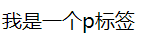
\includegraphics[]{img/C1/1-3/1.png}
\end{figure}

再来看一下经过CSS修饰过后的HTML标签:

\begin{lstlisting}[style=htmlcssjs, title=Hello World!]
p {
    color: red;
    border: 1px solid red;
    width: 140px;
    height: 40px;
}
\end{lstlisting}

\begin{figure}[H]
	\centering
	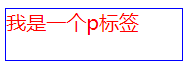
\includegraphics[]{img/C1/1-3/2.png}
\end{figure}

CSS是用来修饰HTML样式的。虽然HTML本身是有一些默认样式,但如果想改变HTML标签的样式,就需要借助CSS。 \\

HTML + CSS构成了网页的基本页面结构和样式。

\begin{lstlisting}[style=htmlcssjs, title=添加样式]
<!DOCTYPE html>
<html lang="en">
<head>
    <meta charset="UTF-8">
    <title>添加样式</title>
    <style type="text/css">
        p {
            font-size: 12px;
            color: #930;
            text-align: center;
        }
    </style>
</head>
<body>
    <p>Hello World!</p>
</body>
</html>
\end{lstlisting}

\newpage

\section{标签}

\subsection{标签}

HTML中标签的语法有以下几点:

\begin{enumerate}
	\item 标签(tag)是由英文尖括号【<】和【>】括起来的,如\lstinline|<html>|就是一个标签??

	\item HTML中的标签一般都是成对出现的,分开始标签和结束标签。结束标签比开始标签多了一个【/】。 \\
	      \begin{lstlisting}[style=htmlcssjs]
<p></p>
<div></div>
<span></span>
    \end{lstlisting}

	\item 标签与标签之间是可以嵌套的,但先后顺序必须保持一致。如,\lstinline|<div>|里嵌套\lstinline|<p>|,那么\lstinline|</p>|必须放在\lstinline|</div>|的前面。 \\
	      \begin{lstlisting}[style=htmlcssjs]
<div><p>Hello World!</p></div>
    \end{lstlisting}

	\item HTML标签不区分大小写,如\lstinline|<h1>|和\lstinline|<H1>|是一样的,但建议小写,因为大部分程序员都已小写为准。
\end{enumerate}

\newpage

\section{HTML文档结构}

\subsection{HTML文档结构}

\begin{lstlisting}[style=htmlcssjs, title=HTML文档结构]
<!DOCTYPE html>
<html lang="en">
<head>
    <meta charset="UTF-8">
    <title>HTML文档结构</title>
</head>
<body>

</body>
</html>
\end{lstlisting}

\begin{itemize}
    \item \lstinline|<!DOCTYPE html>|:文档类型声明,表示该文件为\lstinline|HTML|文件。\lstinline|<!DOCTYPE>|声明必须是\lstinline|HTML|文档的第一行,位于\lstinline|<html>|之前。
    
    \item \lstinline|<html></html>|:\lstinline|<html>|用来标识HTML文档的开始,\lstinline|</html>|位于HTML文档的最后面,用来标识HTML文档的结束。这两个标签对成对存在,中间的部分是文档的头部和主题。
    
    \item \lstinline|<head></head>|:标签包含有关HTML文档的信息,可以包含一些辅助性标签。如\lstinline|<title></title>|、\lstinline|<link />|、\lstinline|<meta />|、\lstinline|<style></style>|、\lstinline|<script></script>|等,浏览器除了会在标题栏显示\lstinline|<title>|元素的内容外,不会向用户显示\lstinline|head|元素内的其他任何内容。
    
    \item \lstinline|<body></body>|:HTML文档的主体部分,在此标签中可以包含\lstinline|<p>|、\lstinline|<h1>|、\lstinline|<br>|等众多标签。\lstinline|<body>|出现在\lstinline|</head>|之后,且必须在闭标签\lstinline|</html>|之前闭合。
\end{itemize}

\newpage

\section{小哥,做头吗?——head标签}

\subsection{head标签}

文档的头部描述了文档的各种属性和信息,包括文档的标题等,绝大多数文档头部包含的数据都不会真正作为内容显示给读者。 \\

\lstinline|head|标签为双标签\lstinline|<head></head>|,表示头部标签,通常用来嵌套\lstinline|meta|、\lstinline|title|、\lstinline|style|等标签。

\begin{itemize}
    \item \lstinline|<title>|:在\lstinline|<title>|和\lstinline|</title>|标签之间的文字内容是网页的标题信息,它会出现在浏览器的标题栏中。网页的\lstinline|<title>|用于告诉用户和搜索引擎这个网页的主要内容是什么,搜索引擎可以通过网页标题,迅速的判断出网页的主题。每个网页的内容都是不同的,每个网页都应该有一个独一无二的title。
    
    \item \lstinline|<meta charset="UTF-8">|:设置当前文件字符编码。
    
    \item \lstinline|<style>|:设置当前文件样式。
\end{itemize}

\newpage

\section{你就是馋人家的身子!——body标签}

\subsection{body标签}

在网页上要展示出来的页面内容一定要放在\lstinline|<body>|中。

\begin{lstlisting}[style=htmlcssjs, title=body标签]
<!DOCTYPE html>
<html lang="en">
<head>
 <meta charset="UTF-8">
 <title>body标签</title>
</head>
<body>
    <!-- 标题标签 -->
    <h1>HTML简介</h1>
    <!-- 段落标签 -->
    <p>HTML的全称为超文本标记语言,是一种标记语言。</p>
    <!-- 段落标签 -->
    <p>它包括一系列标签.可以将网络上的文档格式统一。</p>
</body>
</html>
\end{lstlisting}

\newpage